\documentclass{article}
\usepackage{graphicx} % Required for inserting images
\usepackage{subcaption}
\usepackage{amsmath}
\usepackage{multicol,multirow}


\title{CSE200: Online-1 on \LaTeX}
\author{Utshav Saha (2305077)}
\date{July 2026}

\begin{document}

\maketitle

\section{Introduction}

Document preparation systems are essential for producing structured and professional technical documents. \textbf{LATEX} allows authors to focus on content while maintaining consistent formatting. This article demonstrates formatted text, lists, equations, tables, and figures using commands taught in class.

\subsection{Text Emphasis and Fonts}
This sentence contains \textbf{bold text}, \textit{italic text}, \emph{emphasized text}, and \underline{underlined text}. Font sizes can also vary such as {\Large Large text}, {\small small text}, and {\Huge huge text}.

\section{List Structures}
\subsection{Mixed and Nested List}
\begin{itemize}
    \item Primary Feature
    \item Secondary Features
        \begin{itemize}
    \item[-] Inline Math
    \item[-] Display Math
        \end{itemize}
\end{itemize}

\textbf{Note} Lists can be customized.

\section{Mathematical Modeling}
Mathematical expressions are often used to represent data relationships. Consider variables $x_i, y, \text{ and } z^2.$

\section{Mathematical Modeling}
Mathematical expressions are commonly used to describe relationships among
variables. Let the variables be $x_i$, $y_j$, and $\sigma^2$.

\subsection{Displayed Equations}

\begin{equation}
    y_j = \alpha{x_j}^2 + \beta x_j + \gamma
\end{equation}

\begin{align*}
     T &= \sum_{i=1}^{n}(x_i - \mu)^2 \\
     &= \sum_{i=1}^{n}x_i^2 - 2\mu\sum_{i=1}^{n}x_i + n\mu^2 \\ \tag{2}
\end{align*}

\[
f(x_i) = 
\begin{cases}
    \frac{{x_i}^2}{\sigma^2} & \text{if } x_i \geq 0 \\
    \frac{|x_i|}{\sigma}  & \text{if } x_i < 0 \\
    
\end{cases}
\]

\section{Tabular Data Presentation}

\begin{table}[!h]
    \centering
    \begin{tabular}{|c|c|c|}
    \hline
        \multirow{2}{2cm}{\centering \textbf{Module}} & \multicolumn{2}{|c|}{\textbf{Score}} \\ \cline{2-3}
          & Theory & Lab  \\ \hline
          Module A & 75 & 80 \\ \hline
          \multirow{2}{2cm}{\centering Module B} & 88 & 90 \\
          & 85 & 87 \\ \hline
          Module C & 70 & 72 \\ \hline
          
        
    \end{tabular}
    \caption{Module-wise Performance Summary}
    \label{tab:comparison}
\end{table}

\clearpage

\section{Visual Comparison}
\subsection{Asymmetric Subfigure Layout}
    \begin{figure}[ht]
    \centering
    \begin{subfigure}[b]{0.8\linewidth}
        \centering
        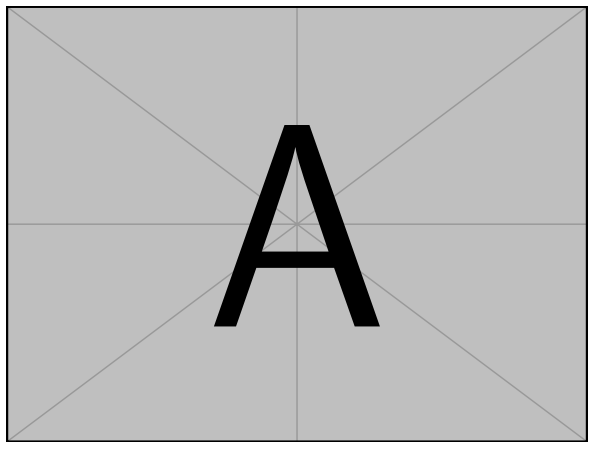
\includegraphics[width=1\linewidth]{A (1).PNG}
        \caption{Main Diagram}
        \label{fig:placeholder}
    \end{subfigure}
    \begin{subfigure}[b]{0.3\linewidth}
        \centering
        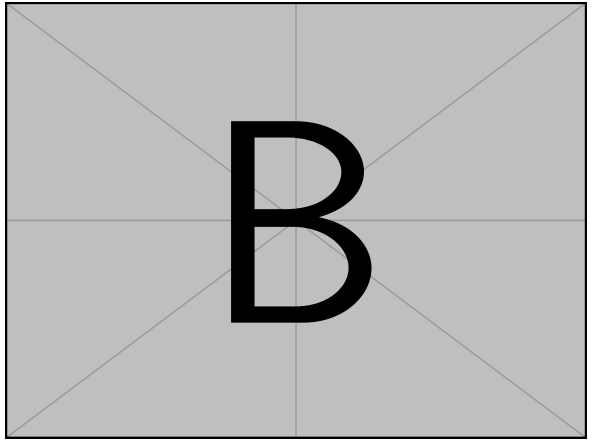
\includegraphics[width=1\linewidth]{B (1).PNG}
        \caption{Detail B}
        \label{fig:placeholder}
    \end{subfigure}
    \hfill
    \begin{subfigure}[b]{0.3\linewidth}
        \centering
        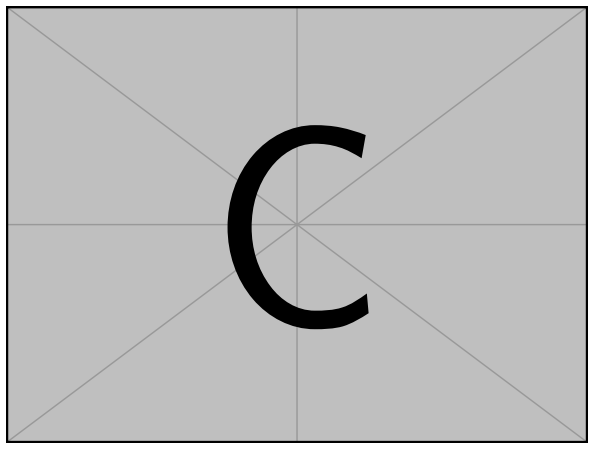
\includegraphics[width=1\linewidth]{C (1).PNG}
        \caption{Detail C}
        \label{fig:placeholder}
    \end{subfigure}
    
    \caption{Asymmetric layout with one dominant figure}
    \label{fig:outputs}
\end{figure}

Figure \ref{fig:outputs} illustrates how visual elements can be arranged systematically within a document.

\section*{Conclusion}
This article highlighted the importance of \textbf{structured writing} using \LaTeX.The use of \textit{formatted text}, mathematical expressions, tables, and figures improves both \underline{readability} and presentation quality.
\end{document}
